\chapter{Sviluppo Android}

\section{Funzionalità base}

Per sviluppare l'applicazione Android è stato utilizzato Android Studio, che consente di sviluppare in linguaggio Java o
Kotlin (consentendo anche di integrare librerie native in C/C++). Per questo progetto si è deciso di utilizzare Java.

Ogni applicazione Android è costituita da un insieme di \textit{Activity}, ovvero oggetti che definiscono il comportamento
dell'interfaccia utente. Queste Activity sono gli Entry Point dell'applicazione, rappresentano i meccanismi con i quali
l'utente può avviare ed interagire con l'applicazione.
Un altro concetto importante nell'ambito dello sviluppo Android è quello del \textit{Lifecycle}. Ogni Activity segue un proprio
ciclo vitale, e il suo comportamento può cambiare a seconda dello stato in cui si trova. Per questo motivo ciascuna Activity
mette a disposizione dei metodi di callback da invocare quando l'Activity transiziona in uno stato particolare del suo 
Lifecycle (metodi \texttt{onCreate()}, \texttt{onPause()}, etc).

\begin{figure}[h!]
    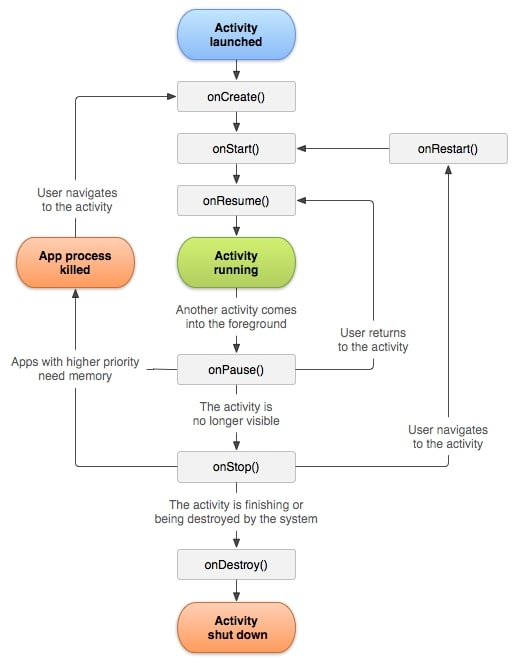
\includegraphics[width=0.45\textwidth]{img/activity_lifecycle.jpg}
    \centering
    \caption{Schema del ciclo vitale di un'activity. \\
    Fonte: https://developer.android.com/guide/components/activities/activity-lifecycle}
    \label{fig:activity_lifecycle}
\end{figure}

Poiché l'applicazione mira alla creazione di video in slow-motion mediante l'interpolazione dei frame, operazione che verrà
svolta in seguito alla cattura del video, distinguiamo due funzionalità principali: 
\textbf{cattura} del video ed \textbf{elaborazione} del video.

\subsection*{Cattura del video}

Activity di riferimento: \texttt{CatturaActivity.java} \\ \\
Per la cattura del video si è fatto affidamento sulle api \textbf{CameraX} di Android, che consentono di utilizzare la 
fotocamera del dispositivo tramite un'interfaccia di alto livello.

CameraX definisce quattro \textit{Use cases}, ciascuno dei quali rappresenta un possibile utilizzo della fotocamera ed è
concretizzato da una classe Java:
\begin{itemize}
    \item \textbf{Preview}: per mostrare un'immagine (o un video) sul display
    \item \textbf{Image analysis}: per applicare vari tipi di algoritmi sulle immagini acquisite
    \item \textbf{Image capture}: per catturare immagini
    \item \textbf{Video capture}: per catturare video (con audio)
\end{itemize}

Per la cattura del video, quindi, si è deciso di combinare una Preview con un Video Capture, in modo da dare la possibilità
all'utente di catturare un video e mostrarne nel frattempo la preview.

Per utilizzare la fotocamera con le api CameraX, è intanto necessario ottenere un oggetto di tipo \texttt{ProcessCameraProvider}, 
ovvero l'istanza della fotocamera. Vediamo di seguito il codice utilizzato per ottenere l'istanza della fotocamera.

\begin{lstlisting}
    provider = ProcessCameraProvider.getInstance(this);
    provider.addListener(() ->
    {
        try {
            ProcessCameraProvider cameraProvider = provider.get();
            startCamera(cameraProvider);
        } catch (Exception e) {
            e.printStackTrace();
        }
    }, getExecutor());
\end{lstlisting}

Si noti che il metodo \texttt{getInstance} restituisce un oggetto di tipo \texttt{ListenableFuture}. Questo perché, per vari
motivi, la fotocamera potrebbe essere attualmente non disponibile. 
È quindi necessario specificare un listener che verrà invocato nel momento in cui la fotocamera si sarà resa disponibile.

Per poter esprimere le sue funzionalità, l'istanza della fotocamera richiede di essere collegata ad un 
\textit{LifecycleOwner}, ovvero un qualsiasi oggetto che possieda un ciclo vitale. In questo modo lo stato della fotocamera 
è vincolato allo stato del LifecycleOwner. Nel nostro caso il LifecycleOwner sarà l'activity su cui stiamo lavorando. 
La funzione \texttt{startCamera} all'interno del listener si occupa di vincolare l'istanza della fotocamera al Lifecycle
dell'attività corrente e agli use case di cui abbiamo bisogno:

\begin{lstlisting}
    private void startCamera(ProcessCameraProvider cameraProvider) {
        cameraProvider.unbindAll();
        CameraSelector camSelector = new CameraSelector.Builder()
                .requireLensFacing(CameraSelector.LENS_FACING_BACK).build();

        Preview preview = new Preview.Builder().build();
        preview.setSurfaceProvider(pview.getSurfaceProvider());

        videoCapt = new VideoCapture.Builder().setVideoFrameRate(25)
                                .setAudioChannelCount(0).build();

        cameraProvider.bindToLifecycle((LifecycleOwner) this, camSelector, preview, videoCapt);
    }
\end{lstlisting}

A questo punto, è possibile utilizzare i controlli della cattura video tramite i metodi \\
\texttt{videoCapture.startRecording()} e \texttt{videoCapture.stopRecording()}

\subsection*{Elaborazione del video}

Activity di riferimento: \texttt{SlomoActivity.java} \\ \\
L'elaborazione del video, come già anticipato, viene affidata al modello Pytorch descritto nel capitolo precedente.

L'elaborazione è computazionalmente pesante e può richiedere tempi di esecuzione di diversi minuti: nei test svolti,
un video di 2 secondi impiegava circa 5 minuti per essere elaborato.
Per questo motivo si è deciso di delegare ad un \textit{Worker} lo svolgimento dell'elaborazione. Ciò consente di disaccoppiare
l'elaborazione dal ciclo vitale dell'activity, eseguendola in parallelo.

\subsubsection*{WorkManager}

La classe Worker fa parte dell'API WorkManager, ovvero l'API raccomandata per il processamento in background su Android.
All'interno della classe Worker, e in particolare nel metodo \texttt{doWork}, è possibile definire il comportamento 
dell'elaborazione che verrà eseguita in background. È stata quindi utilizzata una classe \texttt{SlomoWorker} che estende
Worker.

Per inizializzare un Worker e far partire l'esecuzione in background, è necessario prima creare una WorkRequest,
che può contenere un input da passare all'istanza del Worker. Nel nostro caso, l'unico input che viene passato allo
SlomoWorker è il nome del video da processare.

\begin{lstlisting}
    // Creates WorkRequest, passing videoName as input data
    slomoWorkRequest = new OneTimeWorkRequest.Builder(SlomoWorker.class).
        setInputData(new Data.Builder().putString(SlomoWorker.VIDEO_NAME, videoName).build()).build();
\end{lstlisting}

Per mantenere notificato l'utente dello stato dei progressi dell'elaborazione, si è deciso di introdurre una ProgressBar 
nell'activity. Inoltre, poiché l'elaborazione può richiedere svariati minuti, si è deciso di utilizzare una notifica
Android, anch'essa contenente una ProgressBar. Durante l'elaborazione, il Worker si occupa di notificare i propri progressi
ai componenti in ascolto. È quindi necessario definire una funzione di callback che venga eseguita quando il worker progredisce
nell'elaborazione, notificandolo opportunamente.

\begin{lstlisting}
    WorkManager.getInstance(getApplicationContext())
            .getWorkInfoByIdLiveData(slomoWorkRequest.getId())
            .observeForever(new Observer<WorkInfo>() {
                @Override
                public void onChanged(WorkInfo workInfo) {
                    float progress = workInfo.getProgress()
                            .getFloat(SlomoWorker.PROGRESS_TAG, 0);
                    // gestisce le informazioni ricevute dal worker, aggiornando gli elementi della UI
                    // tra cui le due ProgressBar

                    //...
                    
                    // Remove the observer when not needed anymore
                    // 'this' = observer
                    WorkManager.getInstance(getApplicationContext())
                        .getWorkInfoByIdLiveData(slomoWorkRequest.getId())
                        .removeObserver(this);
                }
            }
\end{lstlisting}

A questo punto possiamo accodare la WorkRequest tra le richieste di lavoro da eseguire:

\begin{lstlisting}
    // Enqueues slomoWorkRequest
    WorkManager.getInstance(this).enqueueUniqueWork(
                            "superSlomoEvaluation",
                            ExistingWorkPolicy.KEEP,
                            slomoWorkRequest);
\end{lstlisting}

La classe SlomoWorker di fatto è poco più che un wrapper per la classe SlowMo, descritta nel capitolo precedente.
Inizialmente, esegue qualche elaborazione preliminare:
\begin{itemize}
    \item Recupera il nome del video passato come input
    \item Recupera i frame estratti dal video
    \item Crea un oggetto di tipo SlowMo
\end{itemize}

Infine, invoca il metodo \texttt{doEvaluation()} sull'oggetto SlowMo, facendo partire di fatto l'elaborazione da parte
del modello.

\section{Conversione video}

L'applicazione necessita di un metodo per convertire i video in immagini contenenti i
fotogrammi, e viceversa convertire le immagini in video una volta finita l'elaborazione.
Si è scelto di usare Ffmpeg, la più diffusa software suite di elaborazione media.

\subsubsection*{FFmpeg}

FFmpeg è il framework multimedia più diffuso sul mercato. Offre la possibilità di convertire, 
registrare, e riprodurre la maggior parte dei formati video e audio. In particolare, 
\textbf{FFmpeg} vero e proprio è la suite di conversione, encoding, e decoding di file
multimediali, nella forma di un programma da linea di comando estremamente flessibile.
\textbf{FFplay} è un media player basato sulle stesse librerie, e \textbf{FFprobe} è un
programma per l'analisi di stream multimediali. Nella maggior parte dei casi, quando si
parla di FFmpeg si intende il programma di conversione di file multimediali.

FFmpeg è gratuito e open source, ed è usato come backend di molte applicazioni di elaborazione
media, sia mobile che desktop. Supporta la maggior parte dei sistemi operativi, tramite librerie
ufficiali o create da utenti terzi, e in particolare, per lo scopo di questo progetto, anche
Android. 

Diverse librerie costituiscono la base di FFmpeg. Le più importanti per la funzione di
conversione sono \emph{libavcodec}, contenente decoder e encoder per molti codec audio e video, 
e \emph{libavformat}, contenente \emph{muxer} e \emph{demuxer} (multiplexer e demultiplexer, 
per l'unione o separazione di canali multimedia) di vari formati media.

L'uso del programma da linea di comando è il seguente: vengono specificati uno o più file di 
input, uno o più file di output, e eventuali filtri e parametri opzionali. Per esempio:

\begin{verbatim}
-- Conversione tra formati audio
ffmpeg -i audioin.wav audioout.mp3
-- Estrazione di fotogrammi come immagini PNG
ffmpeg -i videoin.mp4 frames/%06d.png
-- Uso di filtri video per scalare e ruotare l'immagine, e altri parametri
ffmpeg -i videoin.mp4 -vsync 0 -vf "transpose=1,scale=-1:180" frames/%06d.png
\end{verbatim}

In questo progetto, FFmpeg è stato usato per estrarre i fotogrammi come immagini PNG dal video
di input, e unire i fotogrammi elaborati da Super SlowMo in un video con gli stessi fotogrammi
per secondo dell'originale, e durata quindi raddoppiata.

\subsubsection*{FFmpegKit}

Per poter usare FFmpeg su Android, è stata usata la libreria FFmpegKit, che include strumenti
per eseguire FFmpeg su Android, insieme ad altre piattaforme: iOS, macOS, tvOS, Flutter, e 
React Native. Offre diversi script per fare build delle librerie di FFmpeg, e una libreria 
wrapper per lanciare i comandi di FFmpeg e FFprobe all'interno delle applicazioni. 

Per il contesto di questo progetto, FFmpegKit è stata usata per lanciare i comandi di FFmpeg
all'interno dell'applicazione. Per questo scopo, offre una classe \texttt{FFmpegKit}, che può
essere usata in questo modo, usando come esempio uno dei comandi mostrati sopra:

\begin{lstlisting}
FFmpegSession session = FFmpegKit.execute("-i videoin.mp4 frames/%06d.png");
if (ReturnCode.isSuccess(session.getReturnCode())) {
    Log.i("App", "Extraction success");
} else if (ReturnCode.isCancel(session.getReturnCode())) {
    Log.i("App", "Extraction canceled");
} else {
    Log.d("App", String.format("Extraction failed with state %s and rc %s.%s", session.getState(), session.getReturnCode(), session.getFailStackTrace()));
}
\end{lstlisting}

L'istanza di \texttt{FFmpegSession} offre diversi metodi per ottenere informazioni sulla sessione
in corso, specie nel caso in cui sia creata lanciando il comando in modo asincrono. Per esempio,
questo codice permette di cancellare l'operazione dopo 5 secondi se non ancora conclusa:

\begin{lstlisting}
FFmpegSession session = FFmpegKit.executeAsync("-i videoin.mp4 -vsync 0 -vf \"transpose=1,scale=-1:180\" frames/%06d.png"),
    new FFmpegSessionCompleteCallback() {
        @Override
        public void apply(FFmpegSession session) {
            ReturnCode returnCode = session.getReturnCode();
            Log.i("App", String.format("Extraction success with return code %s", returnCode));
        }
    });
Thread.sleep(5000);
if (session.getState() != SessionState.COMPLETED)
    session.cancel();
\end{lstlisting}

La libreria viene inclusa all'interno del progetto semplicemente aggiungendola a 
\emph{build.gradle}:

\begin{verbatim}
dependencies {
    [...]
    implementation 'com.arthenica:ffmpeg-kit-full:4.5.1-1'
}
\end{verbatim}

\subsubsection*{ConvertVideo}

Per semplificare l'uso di FFmpegKit nel contesto dell'applicazione, e ridurre il rischio
di errori, comandi mal formati, o parametri dimenticati, è stata realizzata un'ulteriore 
classe \texttt{ConvertVideo}, che fa da wrapper a FFmpegKit per aggiungere parametri tramite 
metodi specifici, senza costruire manualmente la stringa del comando.

Un esempio di uso per estrarre fotogrammi, scalarli a 180p, e ruotarli (supponendo quindi un 
video verticale di partenza), è il seguente:

\begin{lstlisting}
convertVideo.rotateClockwise();
convertVideo.setResize(320, 180);
boolean convertSuccess = convertVideo.extractFrames(
    selectedFile,
    extractedFramesDir.getAbsolutePath()
);
\end{lstlisting}

che è equivalente a 

\begin{verbatim}
ffmpeg -i $selectedFile -vsync 0 -vf "transpose=1,scale=320:180" 
    $extractedFramesDir/%06d.png
\end{verbatim}

Questo assicura di evitare errori nell'impostazione dei parametri a livello di compilatore, 
che altrimenti non sarebbero notati fino al tempo di esecuzione data la loro collocazione dentro
ad una stringa.

La classe offre un metodo per estrarre fotogrammi da un video:
\begin{lstlisting}
extractFrames(inVideoPath, outFramesDir)
\end{lstlisting}

e un metodo per unire dei fotogrammi in un video:
\begin{lstlisting}
createVideo(inFramesDir, outVideoPath, fps)
\end{lstlisting}

Offre inoltre alcuni metodi per impostare il ridimensionamento dell'immagine, e la trasposizione,
cioè la rotazione, oltre che metodi per resettare alle impostazioni originali:

\begin{lstlisting}
setResize(int width, int height)
resetResize()
rotateClockwise()
rotateCounterClockwise()
resetRotate()
\end{lstlisting}

La classe viene quindi usata prima e dopo l'elaborazione tramite la classe \texttt{SlowMo}, 
per estrarre i fotogrammi dal video di input e creare il video di output a partire dai
fotogrammi elaborati.

\section{Coordinazione tra processi e activity}

Per riassumere e aggiungere qualche dettaglio, l'applicazione è così strutturata:

\begin{itemize}
    \item \textbf{MainActivity}, contenente un menù di scelta che può avviare:
    \begin{itemize}
        \item \textbf{CatturaActivity}, che si occupa della cattura del video
        \item \textbf{SlomoActivity}, che si occupa dell'elaborazione del video tramite il modello Pytorch
    \end{itemize}
\end{itemize}

La MainActivity è la finestra principale dell'app, mostrata all'avvio, e consente di scegliere quale operazione svolgere
tra cattura video ed elaborazione. La scelta di una delle due operazione si traduce in un passaggio ad una nuova
finestra utente ovvero in un cambio Activity. Questo viene realizzato molto semplicemente tramite degli Intent:

\begin{lstlisting}
    private void showElabora(){
        Intent intent = new Intent(this, SlomoActivity.class);
        startActivity(intent);
    }

    private void showCattura(){
        Intent intent = new Intent(this, CatturaActivity.class);
        startActivity(intent);
    }
\end{lstlisting}

L'activity di cattura è piuttosto semplice, non necessita di processi in background ed è dunque costituita dal solo Thread
della UI. La fotocamera viene agganciata al ciclo vitale dell'Activity come già descritto.

La SlomoActivity, al contrario, fa uso di uno SlomoWorker per realizzare l'elaborazione del video mediante il modello Pytorch.
Questa elaborazione viene eseguita concorrentemente agli eventi della UI, ma produce eventi che vanno a modificare gli elementi
della stessa UI (in particolare le ProgressBar).

L'evento che ci interessa segnalare, in relazione al progresso dell'elaborazione video, è l'avvenuta elaborazione di un 
frame. Per gestire l'aggiornamento della UI a seguito di tale evento, si è deciso di utilizzare un modello
simil \textit{Publisher-Subscriber}. A questo scopo è stata creata un'interfaccia \texttt{IProgressHandler}:

\begin{lstlisting}
    public interface IProgressHandler {
        void publishProgress(float progress);
        void publishProgress(float progress, String message);
    }    
\end{lstlisting}

Questa viene concretizzata nella classe \texttt{SlomoWorkerProgressHandler}. Questa classe si occupa di realizzare la logica
di notifica dei progressi alla UI. Per fare questo, si sfruttano due metodi messi a disposizione appositamente dalla classe
Worker: \texttt{setProgressAsync()} e \texttt{setForegroundAsync()}:

\begin{lstlisting}
    public void publishProgress(float progress) {
        worker.setProgressAsync(new Data.Builder().putFloat(progress_tag, progress).build());
        worker.setForegroundAsync(createForegroundInfo(progress));
    }
\end{lstlisting}

Il metodo setProgressAsync() consente di inviare progressi ad un qualsiasi Listener in ascolto sul Worker, incapsulati in
un oggetto Data (in questo caso contenente solo un float). Come visto nella prima sezione di questo capitolo, il Listener
dello SlomoWorker viene assegnato nella SlomoActivity, e si occupa di aggiornare la ProgressBar.
Il metodo setForegroundAsync(), invece, invia un segnale al sistema Android e consente di aggiornare una notifica esistente
o crearne una nuova. Tramite il metodo \texttt{createForegroundInfo()} ci occupiamo di creare un descrittore della notifica:

\begin{lstlisting}
    protected ForegroundInfo createForegroundInfo(@NonNull float progress) {
        // Build or Update a notification with progress bar

        //...

        Notification notification = new NotificationCompat.Builder(context, context.getString(R.string.notification_channel_id))
                .setContentTitle(title)
                .setTicker(title)
                .setSmallIcon(R.mipmap.ic_launcher_round)
                .setOngoing(true)
                .setOnlyAlertOnce(true)
                .setVisibility(NotificationCompat.VISIBILITY_PUBLIC)
                .setProgress(100, (int)(progress * 100), false)
                .addAction(android.R.drawable.ic_delete, cancel, intent)
                .build();

        return new ForegroundInfo(context.getResources()
                    .getInteger(R.integer.notification_id), notification);
    }
\end{lstlisting}

Un oggetto SlomoWorkerProgressHandler, così composto, viene passato dallo SlomoWorker all'oggetto SlowMo, in modo da
consentire a quest'ultimo di pubblicare i propri progressi al termine dell'elaborazione di ciascun frame:

\begin{lstlisting}
    // SlowMo.java

    public synchronized void doEvaluation() {
        //...

        for (Pair<Tensor, Tensor> sample : videoFrames) {
            //...

            // progressIncrements = 1 / (float)numVideoFrames;
            progress += Math.min(progressIncrements, 1f);

            if(progressHandler != null){
                progressHandler.publishProgress(progress);
            }
        }
    }
\end{lstlisting}


--- inserire magari qualche screen dell'applicazione per mostrare i punti chiave ---

FONTI (METTERE IN BIBLIOGRAFIA)

https://ffmpeg.org/
https://github.com/tanersener/ffmpeg-kit